\documentclass{beamer}


% Load essential packages
\usepackage{hyperref} % Only load once to avoid conflicts
\usepackage{stile}
\usepackage{subcaption}
\usepackage{tcolorbox}
\usepackage[font=scriptsize,skip=1pt]{caption}
\usepackage[T1]{fontenc}
\usepackage{csquotes}
\usepackage[backend=biber, style=authoryear, maxnames=3, minnames=1, abbreviate=false, date=long, url=false, isbn=false, doi=false]{biblatex}
\addbibresource{lecture5/bib.bib} % Ensure this matches your bibliography file name

\interfootnotelinepenalty=10000

\usepackage{latexsym, amsmath, xcolor, multicol, booktabs, calligra}
\usepackage{graphicx, pstricks, listings, stackengine}

% Hyperref setup
\hypersetup{
    hidelinks,
    colorlinks=true,
    linkcolor=black,
    citecolor=blue,
    urlcolor=black
}

% Font theme for Beamer
\usefonttheme[onlymath]{serif}

% Custom definitions
\def\cmd#1{\texttt{\color{red}\footnotesize $\backslash$#1}}
\def\env#1{\texttt{\color{blue}\footnotesize #1}}
\definecolor{deepblue}{rgb}{0,0,0.5}
\definecolor{deepred}{rgb}{0.6,0,0}
\definecolor{deepgreen}{rgb}{0,0.5,0}
\definecolor{halfgray}{gray}{0.55}

% Beamer color settings
\setbeamercolor{block title}{bg=blue!70!white, fg=white}
\setbeamercolor{block body}{bg=blue!10!halfgray, fg=white}
\setbeamercolor{section in head/foot}{fg=white}
\setbeamercolor{subsection in head/foot}{fg=white}
\setbeamercolor{title in head/foot}{fg=white}


% Listings settings for code highlighting
\lstset{
    basicstyle=\ttfamily\small,
    keywordstyle=\bfseries\color{deepblue},
    emphstyle=\ttfamily\color{deepred},
    stringstyle=\color{deepgreen},
    numbers=left,
    numberstyle=\small\color{halfgray},
    rulesepcolor=\color{red!20!green!20!blue!20},
    frame=shadowbox,
}

% Title page info
\author{Freya Rubel}
\title{Trade, Migration and Global Challenges}
\subtitle{Trade and Inequality}
\institute{}
\date{20.11.2025}

\graphicspath{{lecture5/}}

\begin{document}

\begin{frame}
    \titlepage
\end{frame}

\begin{frame}
    \tableofcontents[sectionstyle=show, subsectionstyle=show/shaded/hide, subsubsectionstyle=show/shaded/hide]
\end{frame}
\section{Inequality}
\begin{comment}
\begin{frame}{Unequal and Egalitarian Societies}
    \begin{center}
        \begin{Large}
            In your opinion, what defines an equal/egalitarian society and when would you speak of an unequal society?
        \end{Large}
    \end{center}
\end{frame}
\end{comment}

\begin{frame}{How do we Measure Inequality?}
Ideally, one would like to compare the differences in well-being. \pause \\ Since data on subjective well-being needs to be collected and comparisons between self-reported well-being and happiness are tricky, consumption and income are used as a proxy. 
    \begin{itemize}
        \item Gini Coefficient
        \item Lorenz Curve
        \item Income Share Ratios
        \item Ratio of Median to Mean Income
        \item Relative Poverty Rate and Depth of Poverty
    \end{itemize}
\end{frame}

\begin{frame}{Lorenz Curve - Introduction}
    \begin{figure}
        \centering
        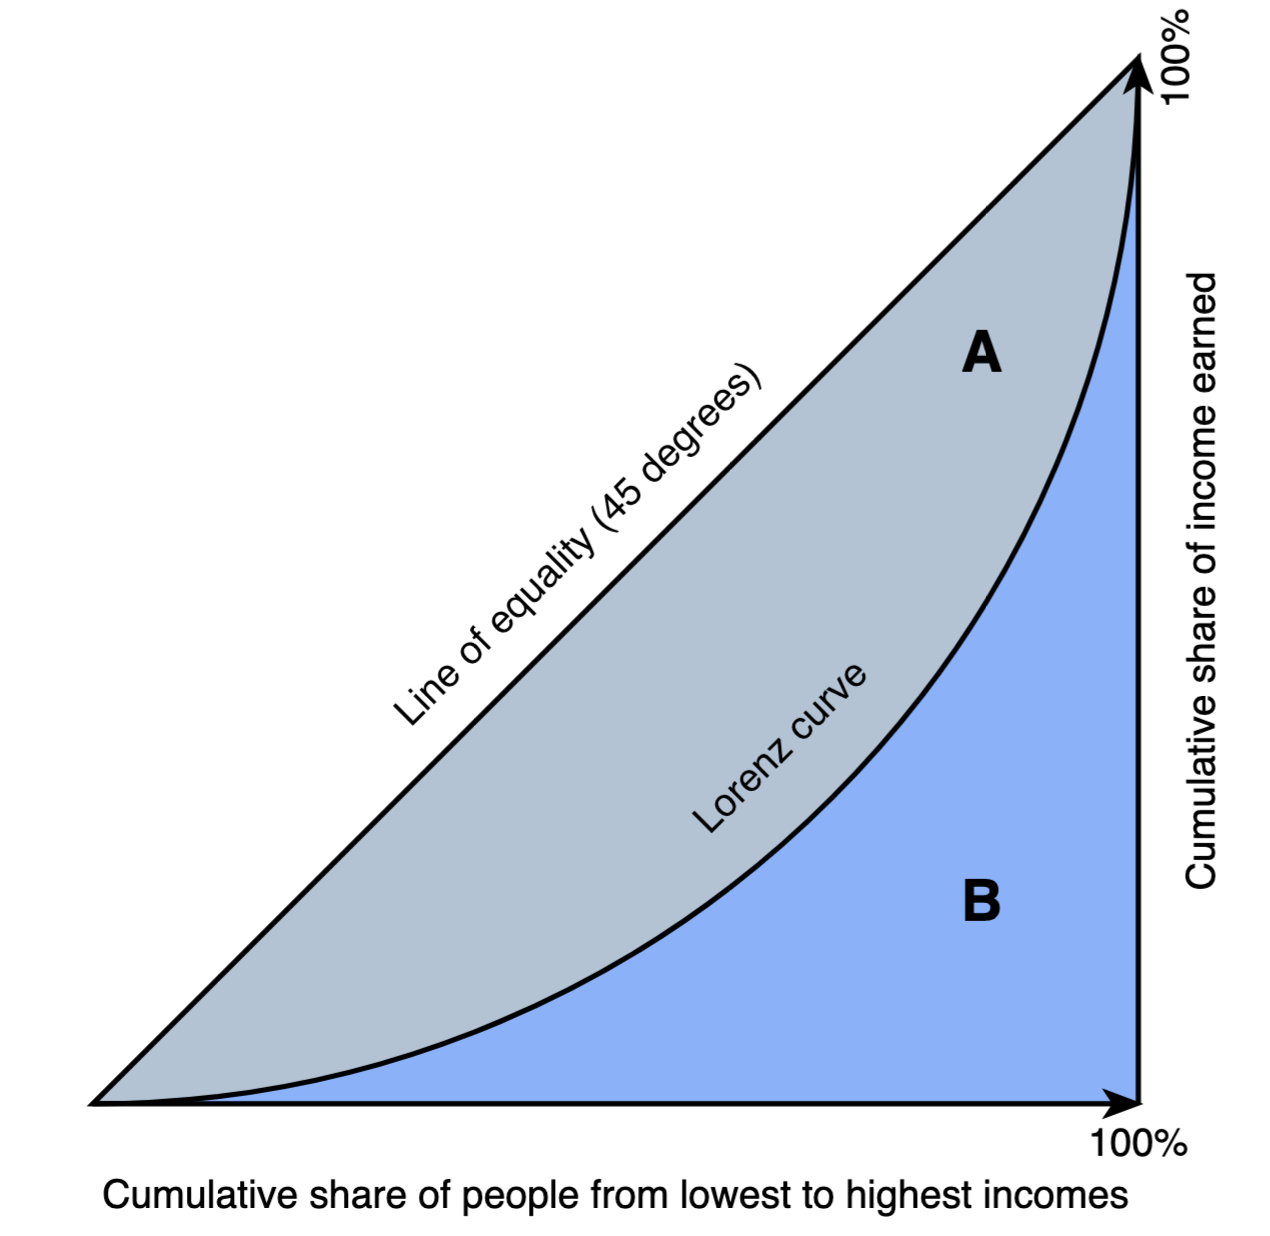
\includegraphics[width=0.6\linewidth]{lorenz curve intro.png}
        \caption{Representative depiction of a Lorenz curve}
        \label{fig:enter-label}
    \end{figure}
\end{frame}

\begin{frame}{Lorenz Curve - Examples}
\textbf{Income Inequality across countries in 2020}
    \begin{figure}
        \centering
        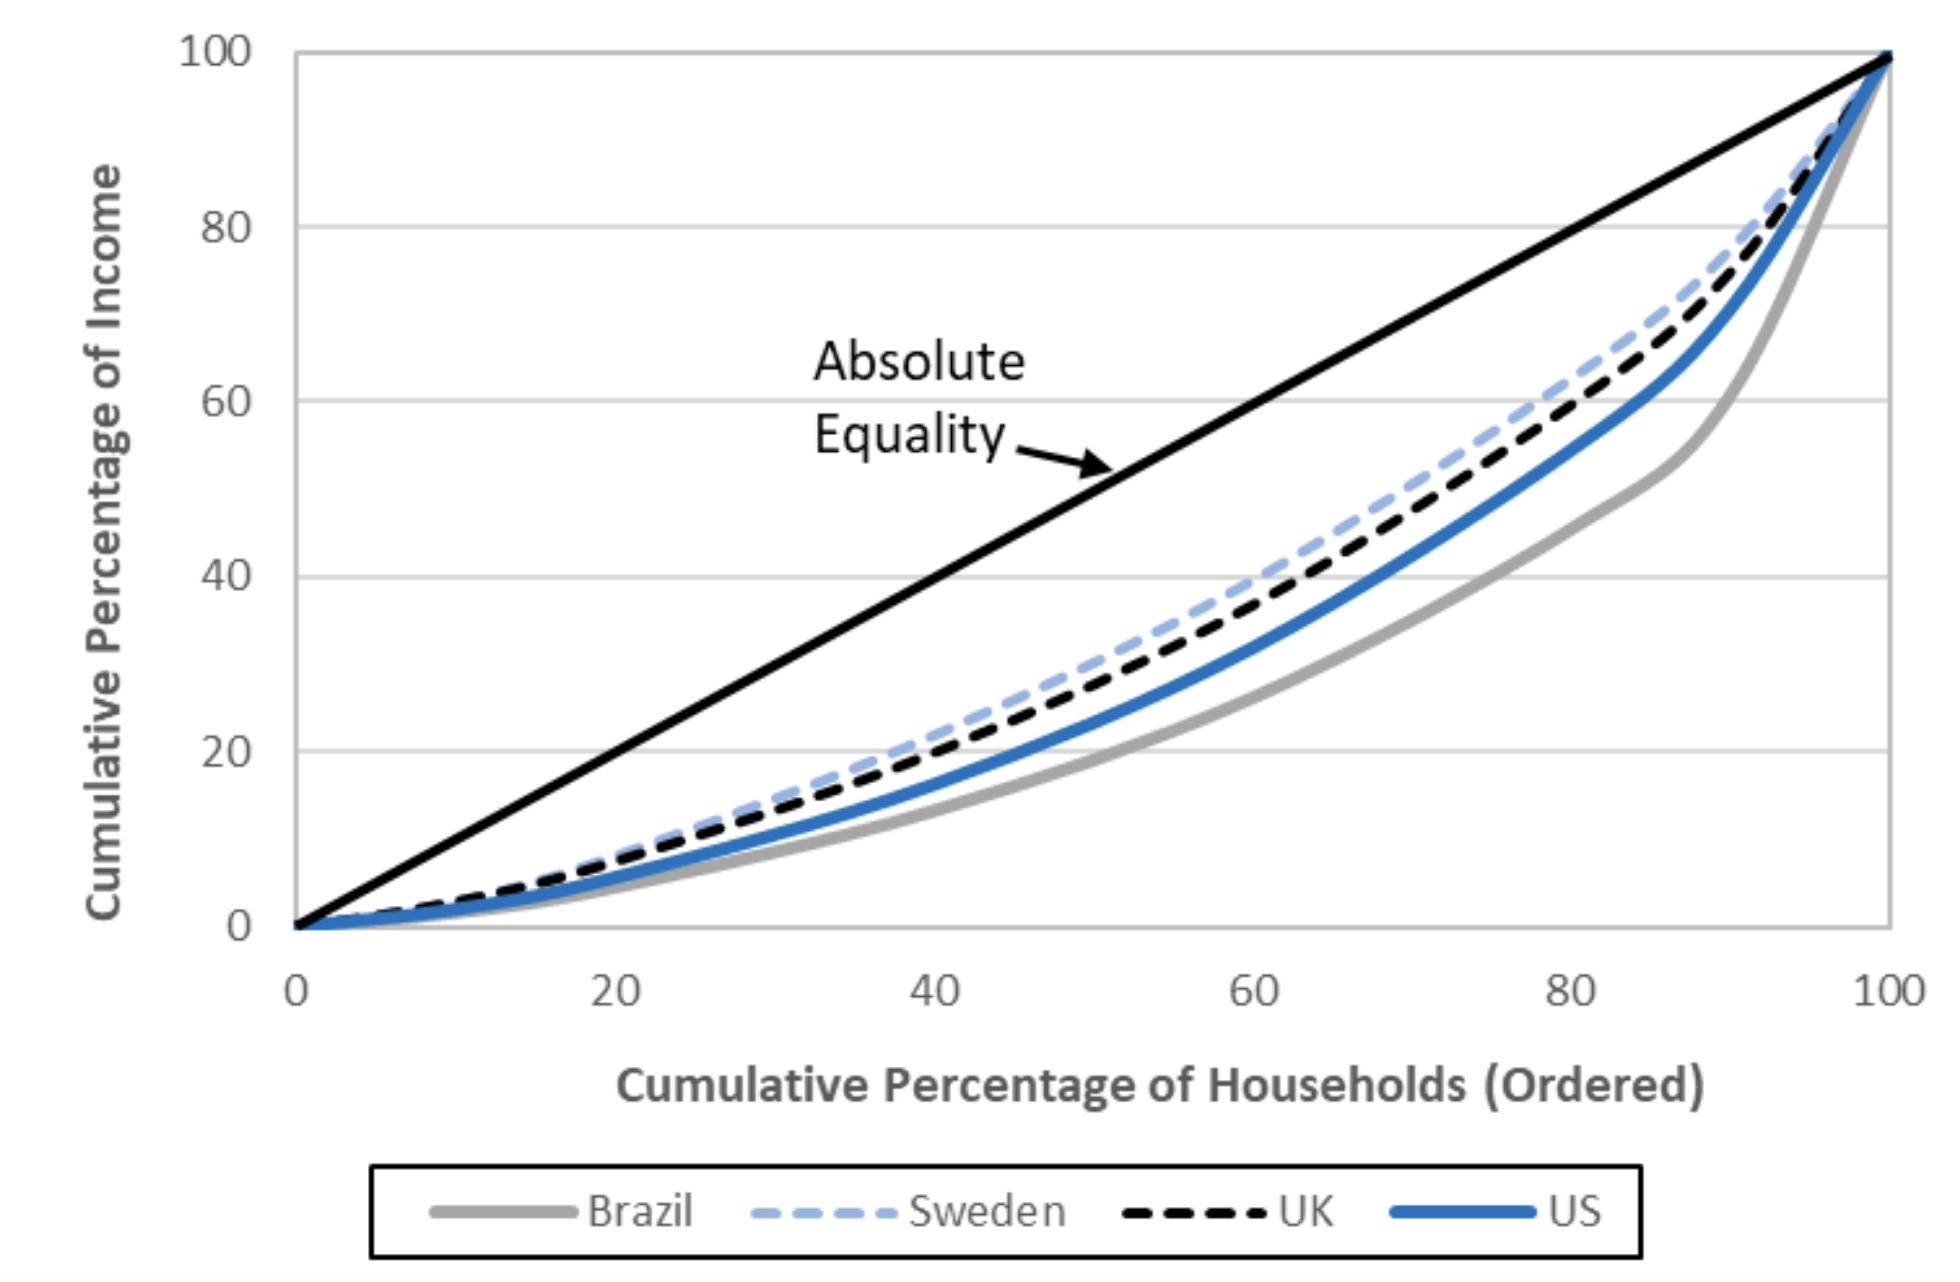
\includegraphics[width=0.8\linewidth]{lorenz_curves_2020.png}
        \caption{Data Source: World Bank. World Development Indicators.}
        \label{fig:enter-label}
    \end{figure}
\end{frame}

\begin{frame}{Gini Coefficient}
    \textbf{Mathematical Formula} \\
    \begin{minipage}[t]{0.5\textwidth} % Adjust width as needed
    \begin{itemize} \footnotesize
        \item $n$ different individuals
        \item $\bar{y}$ is the mean income 
        \item $y_i$ and $y_j$ are two different individuals
    \end{itemize}
\end{minipage}%
\hfill % Adds space between the minipages
\begin{minipage}[t]{0.5\textwidth}
       $$G = \frac{\sum_{i=1}^{n} \sum_{j=1}^{n} |y_i - y_j|}{2n^2 \bar{y}}$$ % you compare each individual to each individual. n^2 comparisons and 2 times that many because you are comparing yi with yj and also yi with yj. dividing by 2n^2 gives you the average difference and y bar makes it scale invariant. YOu wan to measure proportional inequality, not absolute inequality. if one person earns twice as much as another person, we want to evaluate this the same way no matter if the absolute distance between the two is 50,000 or 100,000 dollars
       % absolutely equal society, everyone earns the same -> difference between all pairs is zero, making the numerator 0 and G=0. contrast: one person or household earns all the income in the society or population that you are studying and everyone els earns nothing. The G=
\end{minipage} \vspace{0.15cm}\\
    \textbf{Graphical Formula using the Lorenz Curve}
   \begin{minipage}[t]{0.45\textwidth} % Adjust width as needed
    \begin{figure}[H] % [H] forces placement exactly here, requires the float package
        \centering
        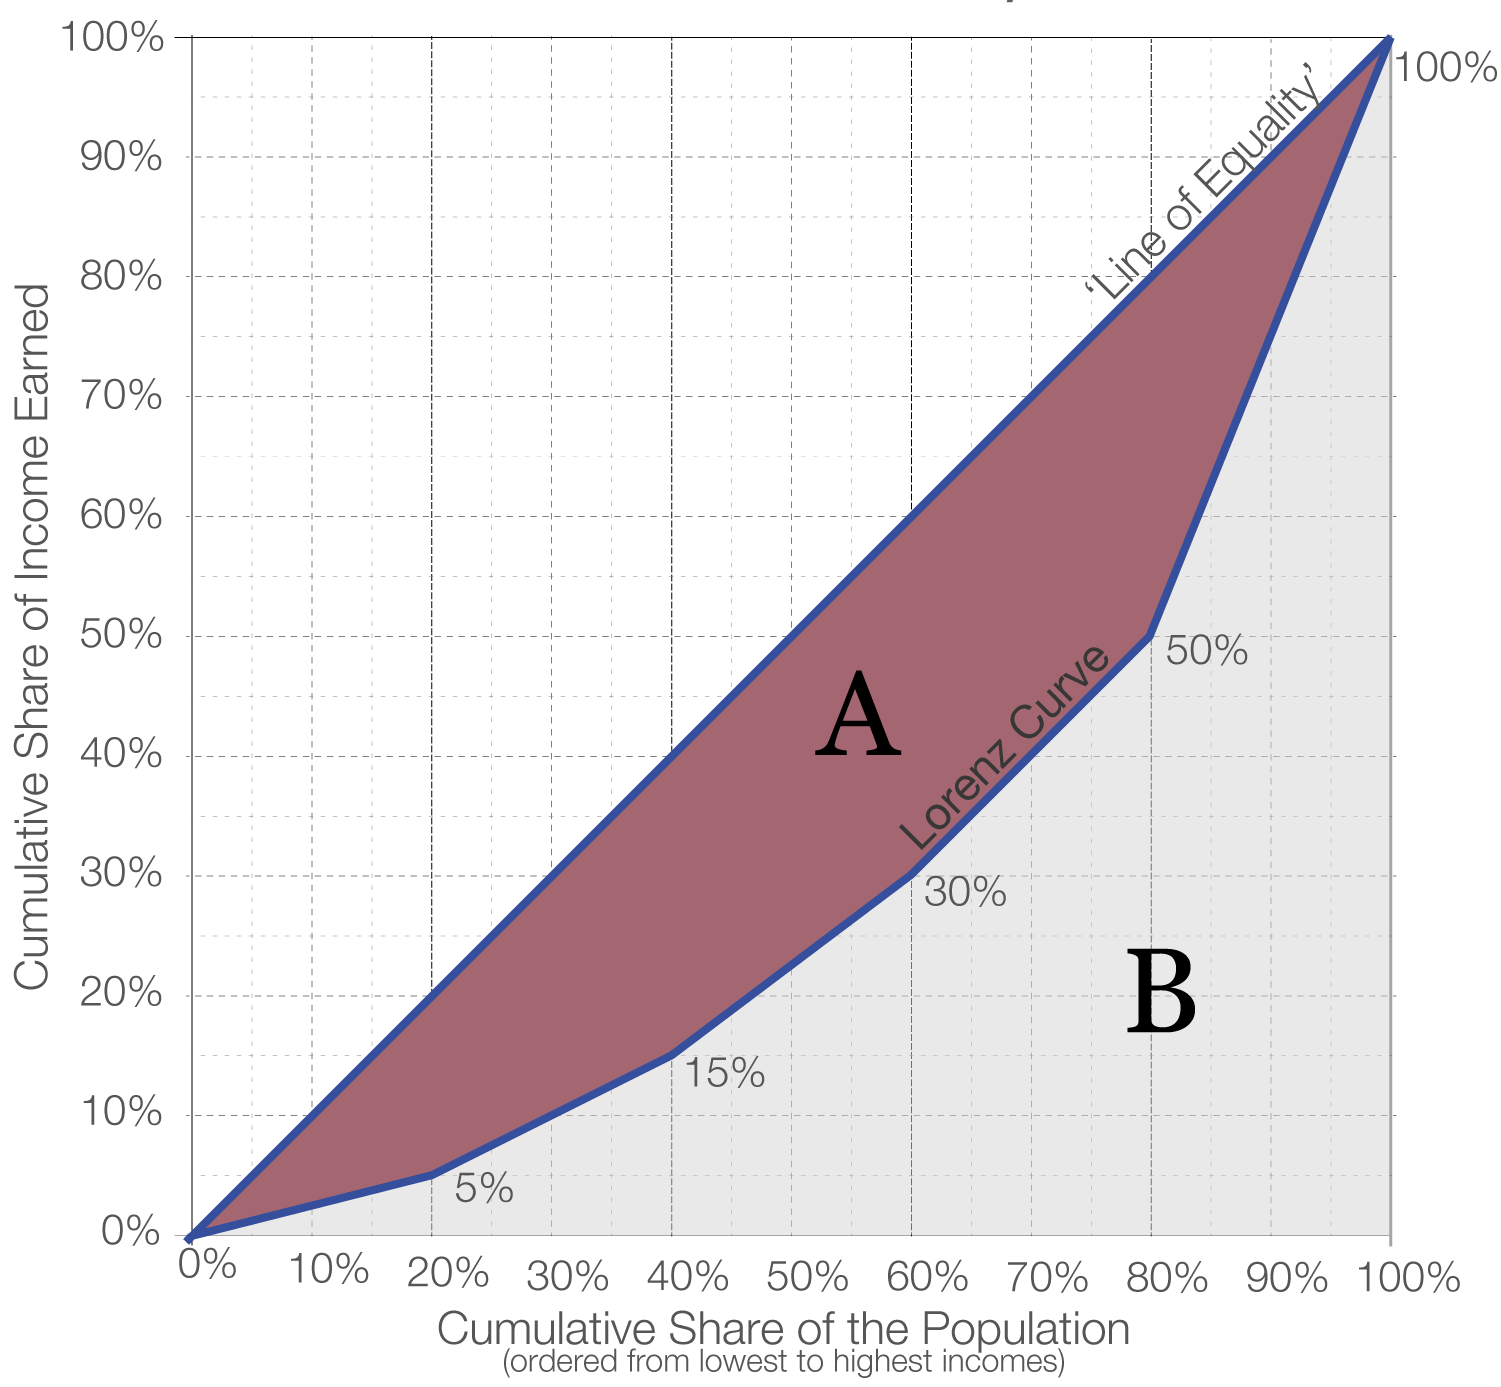
\includegraphics[width=0.8\linewidth]{Gini-measure-schematic-1_3000.png}
        \label{fig:enter-label}
    \end{figure}
\end{minipage}%
\hfill % Adds space between the minipages
\begin{minipage}[t]{0.45\textwidth}
        $$G = \frac{\text{Area A}}{\text{Area A} + \text{Area B}}$$
\end{minipage}
\end{frame}

\begin{frame}{Income Distribution 2023 - Bottom 50\%}
    \begin{figure}
        \centering
        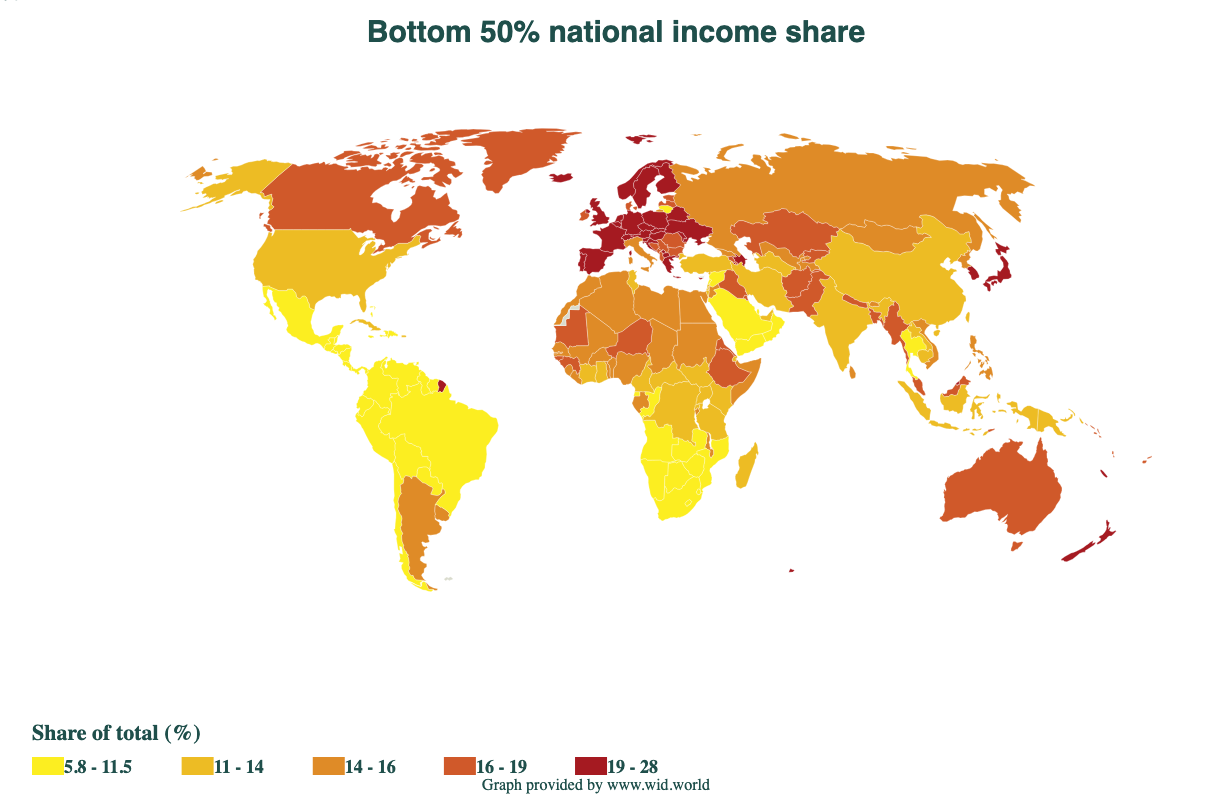
\includegraphics[width=\linewidth]{graph_world_bottom_50.png}
        \caption{Income Share of the bottom 50\%. Source: World Inequality Database.}
        \label{fig:enter-label}
    \end{figure}
\end{frame}

\begin{frame}{Income Distribution 2023 - Top 10\%}
    \begin{figure}
        \centering
        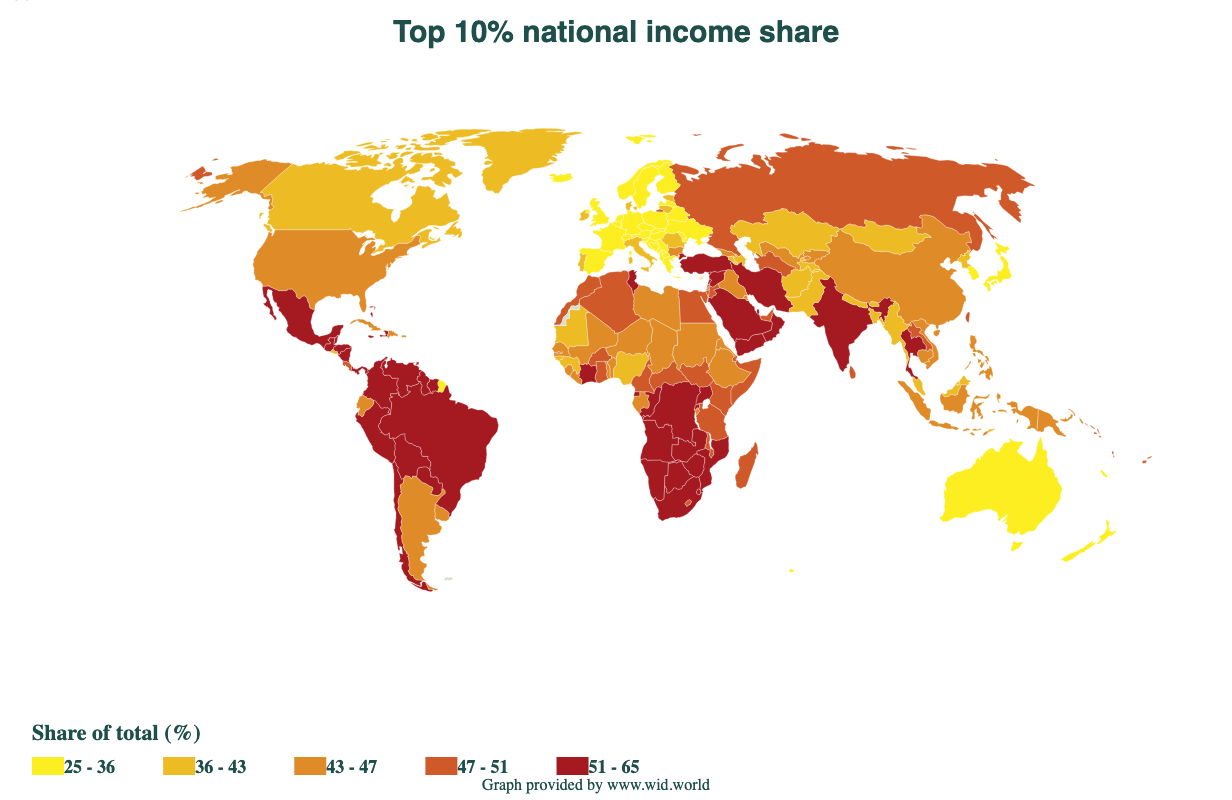
\includegraphics[width=\linewidth]{graph_world_top_10.png}
        \caption{Income Share of the top 10\%. Source: World Inequality Database.}
        \label{fig:enter-label}
    \end{figure}
\end{frame}

\begin{frame}{Income Distribution 2023 - Top 1\%}
    \begin{figure}
        \centering
        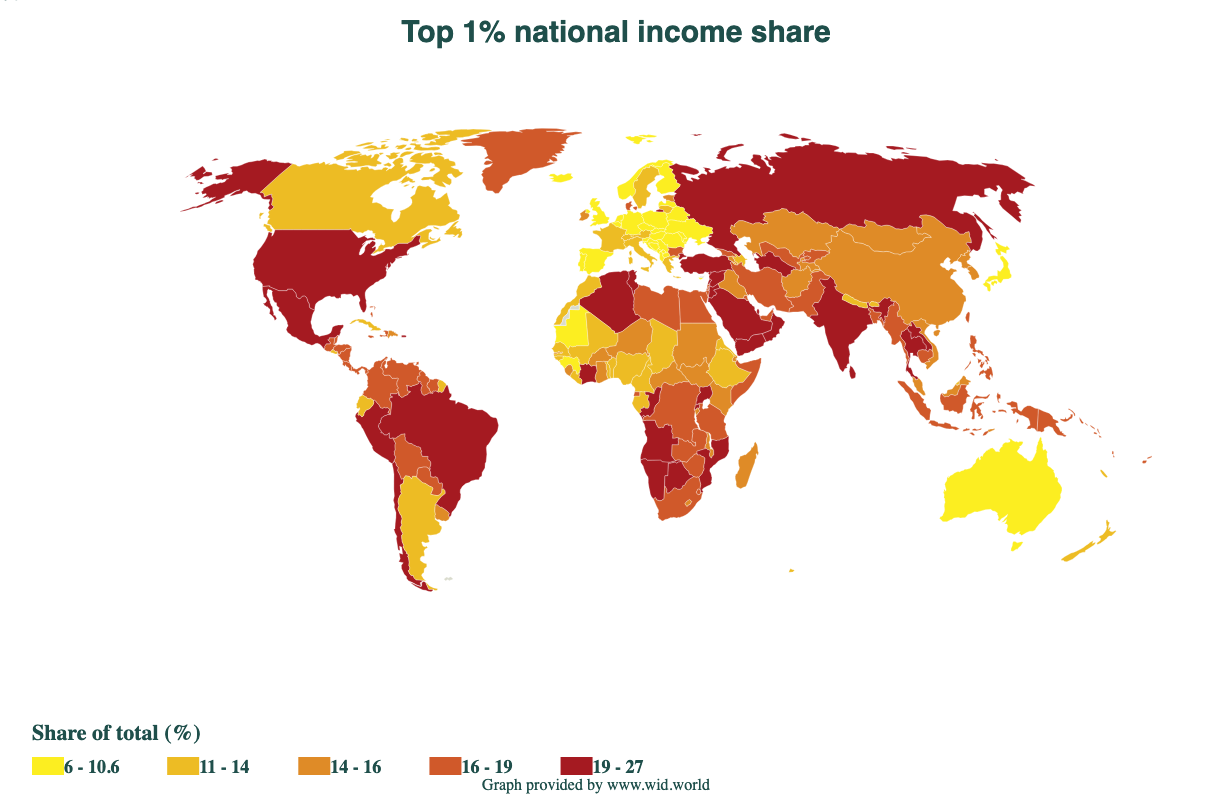
\includegraphics[width=\linewidth]{graph_world_top_1.png}
        \caption{Income Share of the top 1\%. Source: World Inequality Database.}
        \label{fig:enter-label}
    \end{figure}
\end{frame}

\begin{frame}{Income Distribution - Normal}
\begin{figure}
    \centering
    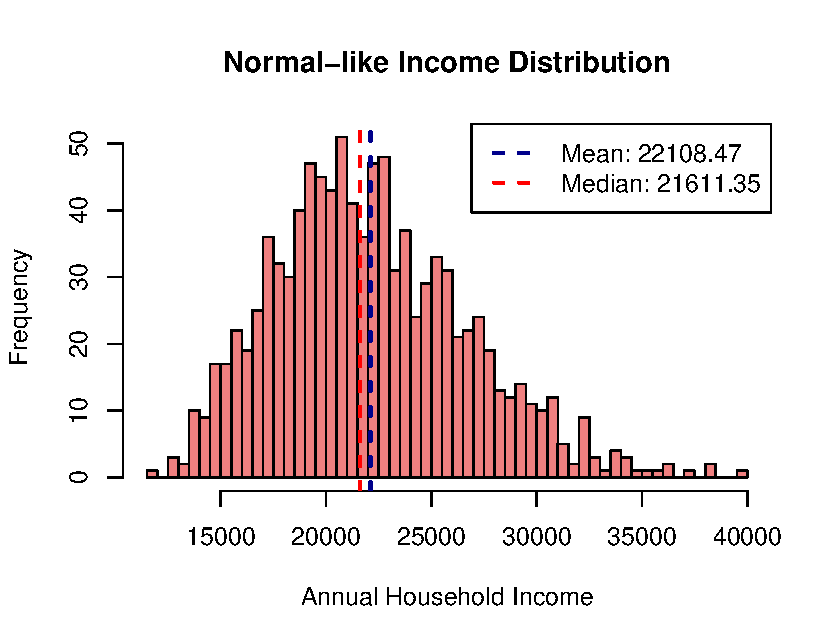
\includegraphics[width=0.9\linewidth]{normal_income_distribution.pdf}
    \caption{Normal-like Income Distribution}
    \label{fig:enter-label}
\end{figure}
\end{frame}

\begin{frame}{Income Distribution - Skewed}
\begin{figure}
    \centering
    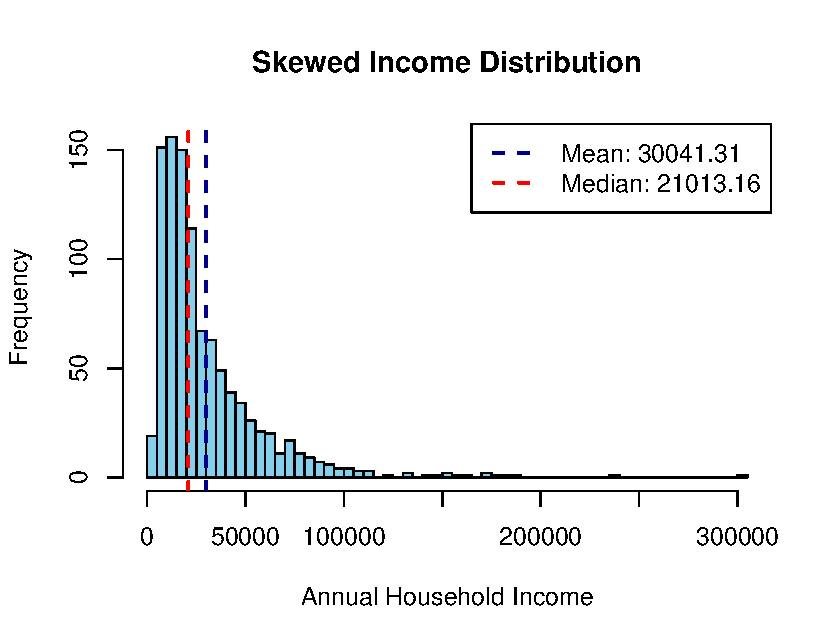
\includegraphics[width=0.9\linewidth]{skewed_income_distribution.pdf}
    \caption{Skewed Income Distribution}
    \label{fig:enter-label}
\end{figure}
\end{frame}

\begin{frame}{Relative Poverty Rate}
    The poverty rate is measured as the share of individuals that live in a household below the poverty line. Most developed countries use a relative poverty line instead of an absolute poverty line. \\
    \textbf{Example EU:} Line at 60\% of the median annual net equalized income of the population. 
    \begin{itemize}
        \item Thereby, the poverty rate is identifying the people \textit{left behind}. 
        \item Increasing income inequality typically increases the poverty rate even if the median income stays constant.
    \end{itemize}
\end{frame}

\begin{frame}{Relative Poverty Rate - Visualization}
Two societies with the same median income and same poverty line can have very different poverty rates depending on their level of inequality.
    \begin{figure}[ht]
    \centering
    % First subfigure on the left
    \begin{subfigure}[b]{0.49\textwidth}
        \centering
        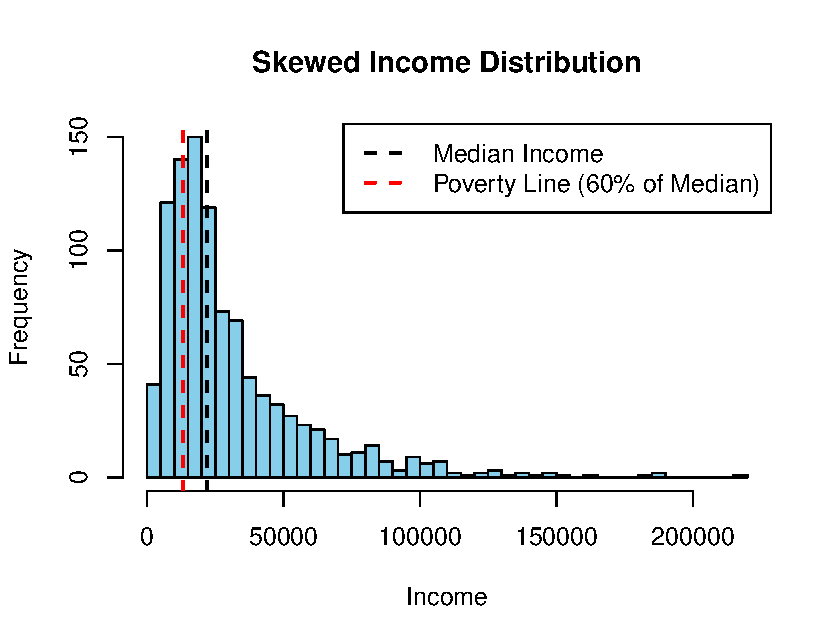
\includegraphics[width=\textwidth]{inequality and poverty.pdf}
        \label{fig:skewed}
    \end{subfigure}
    \hfill
    % Second subfigure on the right
    \begin{subfigure}[b]{0.49\textwidth}
        \centering
        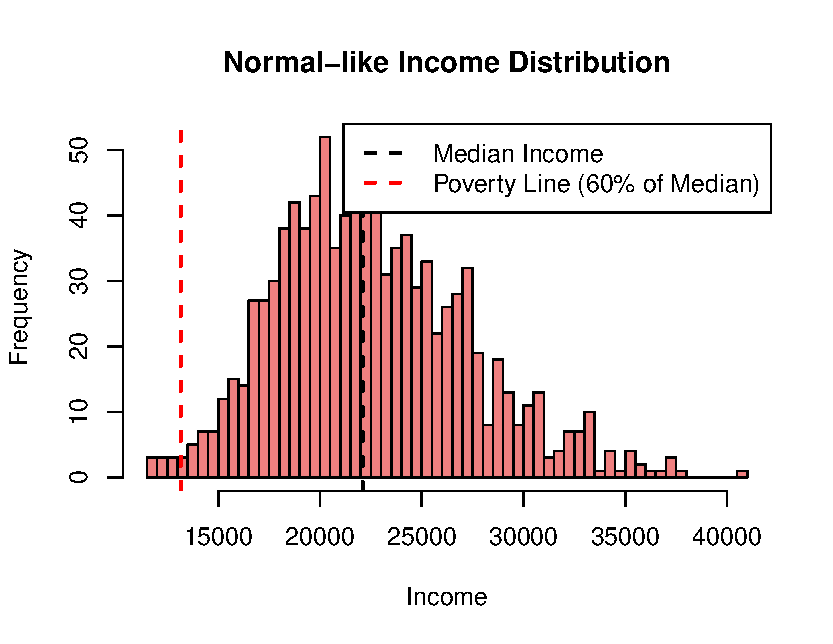
\includegraphics[width=\textwidth]{low_inequality and poverty.pdf}
        \label{fig:normal_like}
    \end{subfigure}
    \caption{Comparison of poverty rate in equal and unequal societies}
    \label{fig:income_distributions}
\end{figure}
\end{frame}

\section{Theory of Trade affecting Inequality}
\begin{frame}{The Comparative Advantage}
    \textbf{Concept:} The comparative advantage is the idea that countries specialize in producing goods they can produce more (cost-)efficiently than others.
    \begin{itemize} \small
        \item Countries trade to exploit these efficiencies, benefiting all participants on a macro level.
        \item \textbf{Example:} 
        \begin{itemize} \footnotesize
            \item \textbf{Country A} specializes in agriculture due to its fertile land.
            \item \textbf{Country B} specializes in manufacturing due to advanced technology.
        \end{itemize}
        \item \textbf{Impact on Inequality:} Specialization can improve overall income but may lead to sectoral imbalances within countries. \\
        \textit{Question:} What happens to the workers employed in manufacturing in Country A and the workers specialized in agriculture in Country B? 
    \end{itemize}
\end{frame}

\begin{frame}{Sectoral Shifts and Employment}
    \begin{itemize}
        \item Trade causes certain sectors to expand while others contract, leading to shifts in employment.
        \item \textbf{Example:} The decline of manufacturing jobs in the U.S. as production shifts to lower-cost countries.
        \item \textbf{Impact:} Workers in declining sectors may face job losses, stagnant wages, or need to transition to new industries.
    \end{itemize}
\end{frame}

\begin{frame}{Heckscher-Ohlin Model}
    \textbf{Concept:} The Heckscher-Ohlin (H-O) model suggests that countries export goods that intensively use their abundant factors of production. Essentially, their factor endowment determines which goods are imported and which get exported.
    \begin{itemize}
        \item Countries with abundant labor export labor-intensive goods; those with abundant capital export capital-intensive goods.
        \item \textbf{Example:} Norway (natural resource abundant) exports oil and gas, while Taiwan (skilled labor abundant) exports advanced electronics.
        \item \textbf{Factor Price Equalization:} Under ideal conditions, trade tends to equalize wages and returns to factors across countries.
    \end{itemize}
    \textbf{BUT} empirical evidence cannot affirm this theory. We do not see an equivalization in factor prices. 
\end{frame}

\begin{frame}{Wage Inequality through Spezialization}
    \begin{itemize}
        \item Historically, trade tends to increase demand for skilled labor in developed countries and for unskilled labor in developing countries.
        \item \textbf{Example:} In the U.S., high-skill jobs (e.g., tech) grow faster than low-skill manufacturing jobs, widening wage gaps.
        \item \textbf{Impact:} Trade can increase wage inequality within countries as high-skill wages rise faster than low-skill wages.
    \end{itemize}
\end{frame}

\begin{frame}{Global Value Chains (GVCs)} % technically doesn't fall under the concept of trade on goods, since these are intermediate goods
\begin{itemize}
        \item GVCs fragment production across countries, creating high-value jobs in some regions and low-wage jobs in others. Specialization raises overall productivity.
        \item \textbf{Example:} Smartphones are designed in high-wage countries and assembled in lower-wage countries.
        \item \textbf{Impact:} While GVCs raise global production, they may exacerbate income inequality across countries.
    \end{itemize}
\end{frame}

\begin{frame}{Outsourcing}
    \textbf{Definition:} Business practice of contracting certain tasks or services to external firms rather than handling them in-house.
    \begin{itemize} \small
        \item \textbf{Purpose:} Reduce costs, improve efficiency, or use specialized skills.
        \item \textbf{Types of Outsourcing:}
        \begin{itemize} \footnotesize
            \item \textbf{Business Process Outsourcing (BPO):} Contracting non-core functions, such as customer service or payroll.
            \item \textbf{IT Outsourcing:} Engaging third-party providers for IT services, including software development and infrastructure.
            \item \textbf{Manufacturing Outsourcing:} Contracting production to external companies, often in countries or regions with lower labor costs.
        \end{itemize}
    \end{itemize}
    \textbf{Impact on Inequality:}
    \begin{itemize} \small
        \item Increases demand for lower-cost labor in outsourcing destinations, raising incomes there.
        \item Can lead to job losses or wage suppression in higher-cost regions, impacting lower-wage, less-skilled workers most.
    \end{itemize}
\end{frame}

\begin{frame}{Offshoring}
    \textbf{Definition:} Practice of relocating certain business processes or production to another country to take advantage of lower costs or other favorable conditions.
    \begin{itemize} \small
        \item Often includes relocating manufacturing, software development, and other labor-intensive tasks.
        \item Distinction from Outsourcing: Offshoring can involve a company’s own facilities abroad, while outsourcing involves contracting external firms.
    \end{itemize}
    %\textbf{Types of Offshoring:}
    %\begin{itemize} \small
     %   \item \textbf{Nearshoring:} Moving production or services to a nearby country, often within the same region.
      %  \begin{itemize} \footnotesize
       %     \item \textbf{Advantages:} Geographic proximity allows for easier collaboration, shorter supply chains, and reduced shipping times.
    %    \end{itemize}
     %   \item \textbf{Farshoring:} Relocating operations to distant countries, often with significantly lower costs.
      %  \begin{itemize} \footnotesize
       %     \item \textbf{Example:} European companies farshoring IT services to India or China for substantial cost savings.
        %    \item \textbf{Challenges:} Cultural and language differences, longer lead times, and potential supply chain vulnerabilities.
        %\end{itemize}
    %\end{itemize}
    \textbf{Impact on Inequality:}
    \begin{itemize} \small
        \item Provides opportunities for low-cost labor markets, raising wages of low-skilled workers in the country that the task is offshored to.
        \item However, it can increase inequality in the country with a reduced demand for lower-skilled domestic jobs and suppress wages in affected industries.
    \end{itemize}
\end{frame}

\begin{comment}
    
\begin{frame}{Group Work (10 Minutes)}
    \textbf{Instructions:}
    \begin{enumerate}
        \item Divide into groups of 3-4 people. Each group will represent one of the following perspectives:
        \begin{itemize} \footnotesize
            \item \textbf{Low-skilled workers in country A} 
            \item \textbf{Skilled workers and professionals in country A} 
        \item \textbf{Low-skilled workers in country B} 
            \item \textbf{Skilled workers and professionals in country B} 
        \end{itemize}
        \item \textbf{Task:} 
        \begin{itemize} \small
            \item Discuss how increased exports from country B to country A in goods produced by low-skilled workers affects your assigned group. 
            \item Identify one \textbf{positive effect} and one \textbf{challenge} that this "shock" in increased trade poses for your group.
            \item Propose one \textbf{policy or action} that could help mitigate negative impacts or enhance positive effects for your group.
        \end{itemize}
        \end{enumerate}
\end{frame}
\end{comment}


\section{Paper Presentation}
\begin{frame}{Autor, Dorn, \& Hanson (2013)}
    \begin{center}
        \begin{Large}
            The China Syndrome: Local Labor Market Effects of Import Competition in the United States \vspace{0.1cm}\\
        \end{Large}
        \begin{large}
            By David H. Autor, David Dorn, and Gordon H. Hanson \\
        \end{large}
        Published in American Economic Review in 2013
    \end{center}
\end{frame}

% Slide 1 - Background
\begin{frame}{Background}
    \begin{itemize}
        \item \textbf{Context}: In the 1990s, China's economy rapidly industrialized, becoming a major exporter of (low-cost) goods.
        \item \textbf{U.S. Trade Shifts}: The share of U.S. imports from China increased drastically, especially post-WTO accession in 2001.
        \item \textbf{Labor Market}: U.S. manufacturing employment fell sharply, with some regions experiencing higher exposure to Chinese imports.
    \end{itemize}
\end{frame}

% Slide 2 - Research Question
\begin{frame}{Research Question}
\begin{tcolorbox}
    \textbf{Main Question}: How has Chinese import competition affected U.S. local labor markets between 1990 and 2007?
\end{tcolorbox}
    \begin{itemize}
        \item \textbf{Key Areas of Impact}: 
        \begin{itemize}
            \item Employment and wage levels in U.S. manufacturing
            \item Labor force participation and unemployment rates
            \item Transfer payments (e.g., unemployment and disability benefits)
        \end{itemize}
        \item \textbf{Hypothesis}: Regions with higher exposure to Chinese imports would experience greater job and wage losses, especially in manufacturing.
    \end{itemize}
\end{frame}

% Slide 3 - Economic Theory
\begin{frame}{Economic Theory}
    \textbf{Comparative Advantage}: China specializes in labor-intensive goods due to its lower labor costs. \\
   \textbf{Heckscher-Ohlin Model}: Predicts that countries will export goods that intensively use their abundant resources. \\
   \textbf{Labor Market Effects}: Theory suggests that import competition will reduce demand for certain types of labor in the importing countries, thereby affecting wages and employment.
\end{frame}

% Slide 4 - Data Sources
\begin{frame}{Data Sources}
\textbf{Import Data}:
    \begin{itemize}
        \item U.N. Comtrade Database, six-digit HS codes for detailed product-level imports from China to the U.S. and other high-income countries.
        \end{itemize}    
    \textbf{Labor Market Data}: 
        \begin{itemize}
            \item Census data (IPUMS) for employment, demographics, wages by Commuting Zone (CZ). Commuting zones are self-constructed: 722 CZs.
            \item American Community Survey for 2006-2008 estimates
        \end{itemize}
    \textbf{Transfer Payments Data}: 
    \begin{itemize}
        \item Bureau of Economic Analysis and Social Security Administration records on benefits by region.
    \end{itemize}
\end{frame}

% Slide 5 - Methodology Overview
\begin{frame}{Methodology Overview}
The authors' identification of a causal impact relies on the regional variation in exposure to the competition from abroad.
    \begin{itemize}
        \item \textcite{china_syndrome} exploit the pre-existing industry composition and specialization prior to the trade shock as a measure of exposure to the competition from abroad.
        \item \textbf{Instrumental Variables (IV) approach}: The growth in Chinese imports to the US are instrumented by the growth in Chinese imports to other high-income countries. 
        \item \textbf{Outcome Variables}: Changes in manufacturing employment, wages, and transfer payments.
    \end{itemize}
\end{frame}

% Slide 6 - Key Variables
\begin{frame}{Key Variables and Measurement}
    \begin{itemize}
        \item \textbf{Import Exposure}: Change in Chinese import exposure per worker in a commuting zone, adjusted by industry employment.
        \item \textbf{Labor Market Outcomes}: Employment levels, labor force participation, and wage changes across sectors.
        \item \textbf{Social Transfers}: Uptake of unemployment, disability, welfare, and other public benefits.
        \item \textbf{Control Variables}: commuting zone demographics, initial employment levels, and start-of-period industry specialization.
    \end{itemize}
\end{frame}

\begin{comment}

\begin{frame}{Empirical Strategy: Instrumental Variables (IV) Approach}
    \begin{itemize}
        \item \textbf{Justification}: Direct measures of U.S. import demand might be endogenous (correlated with the outcome variables that we are trying to observe). An instrument isolates China’s supply-side growth and should only capture the part of the instrument that is due to a growth in Chinese productivity and not due to US demand.
        \item \textbf{IV Construction}: Non-U.S. import growth from China to capture exogenous changes in Chinese export competitiveness.
        \item \textbf{Identifying Assumption}: Growth in imports in other high-income countries is exogenous to U.S. local labor market conditions.
    \end{itemize}

\end{frame}
\end{comment}

\begin{frame}{Scatterplot}
    \begin{figure}
        \centering
        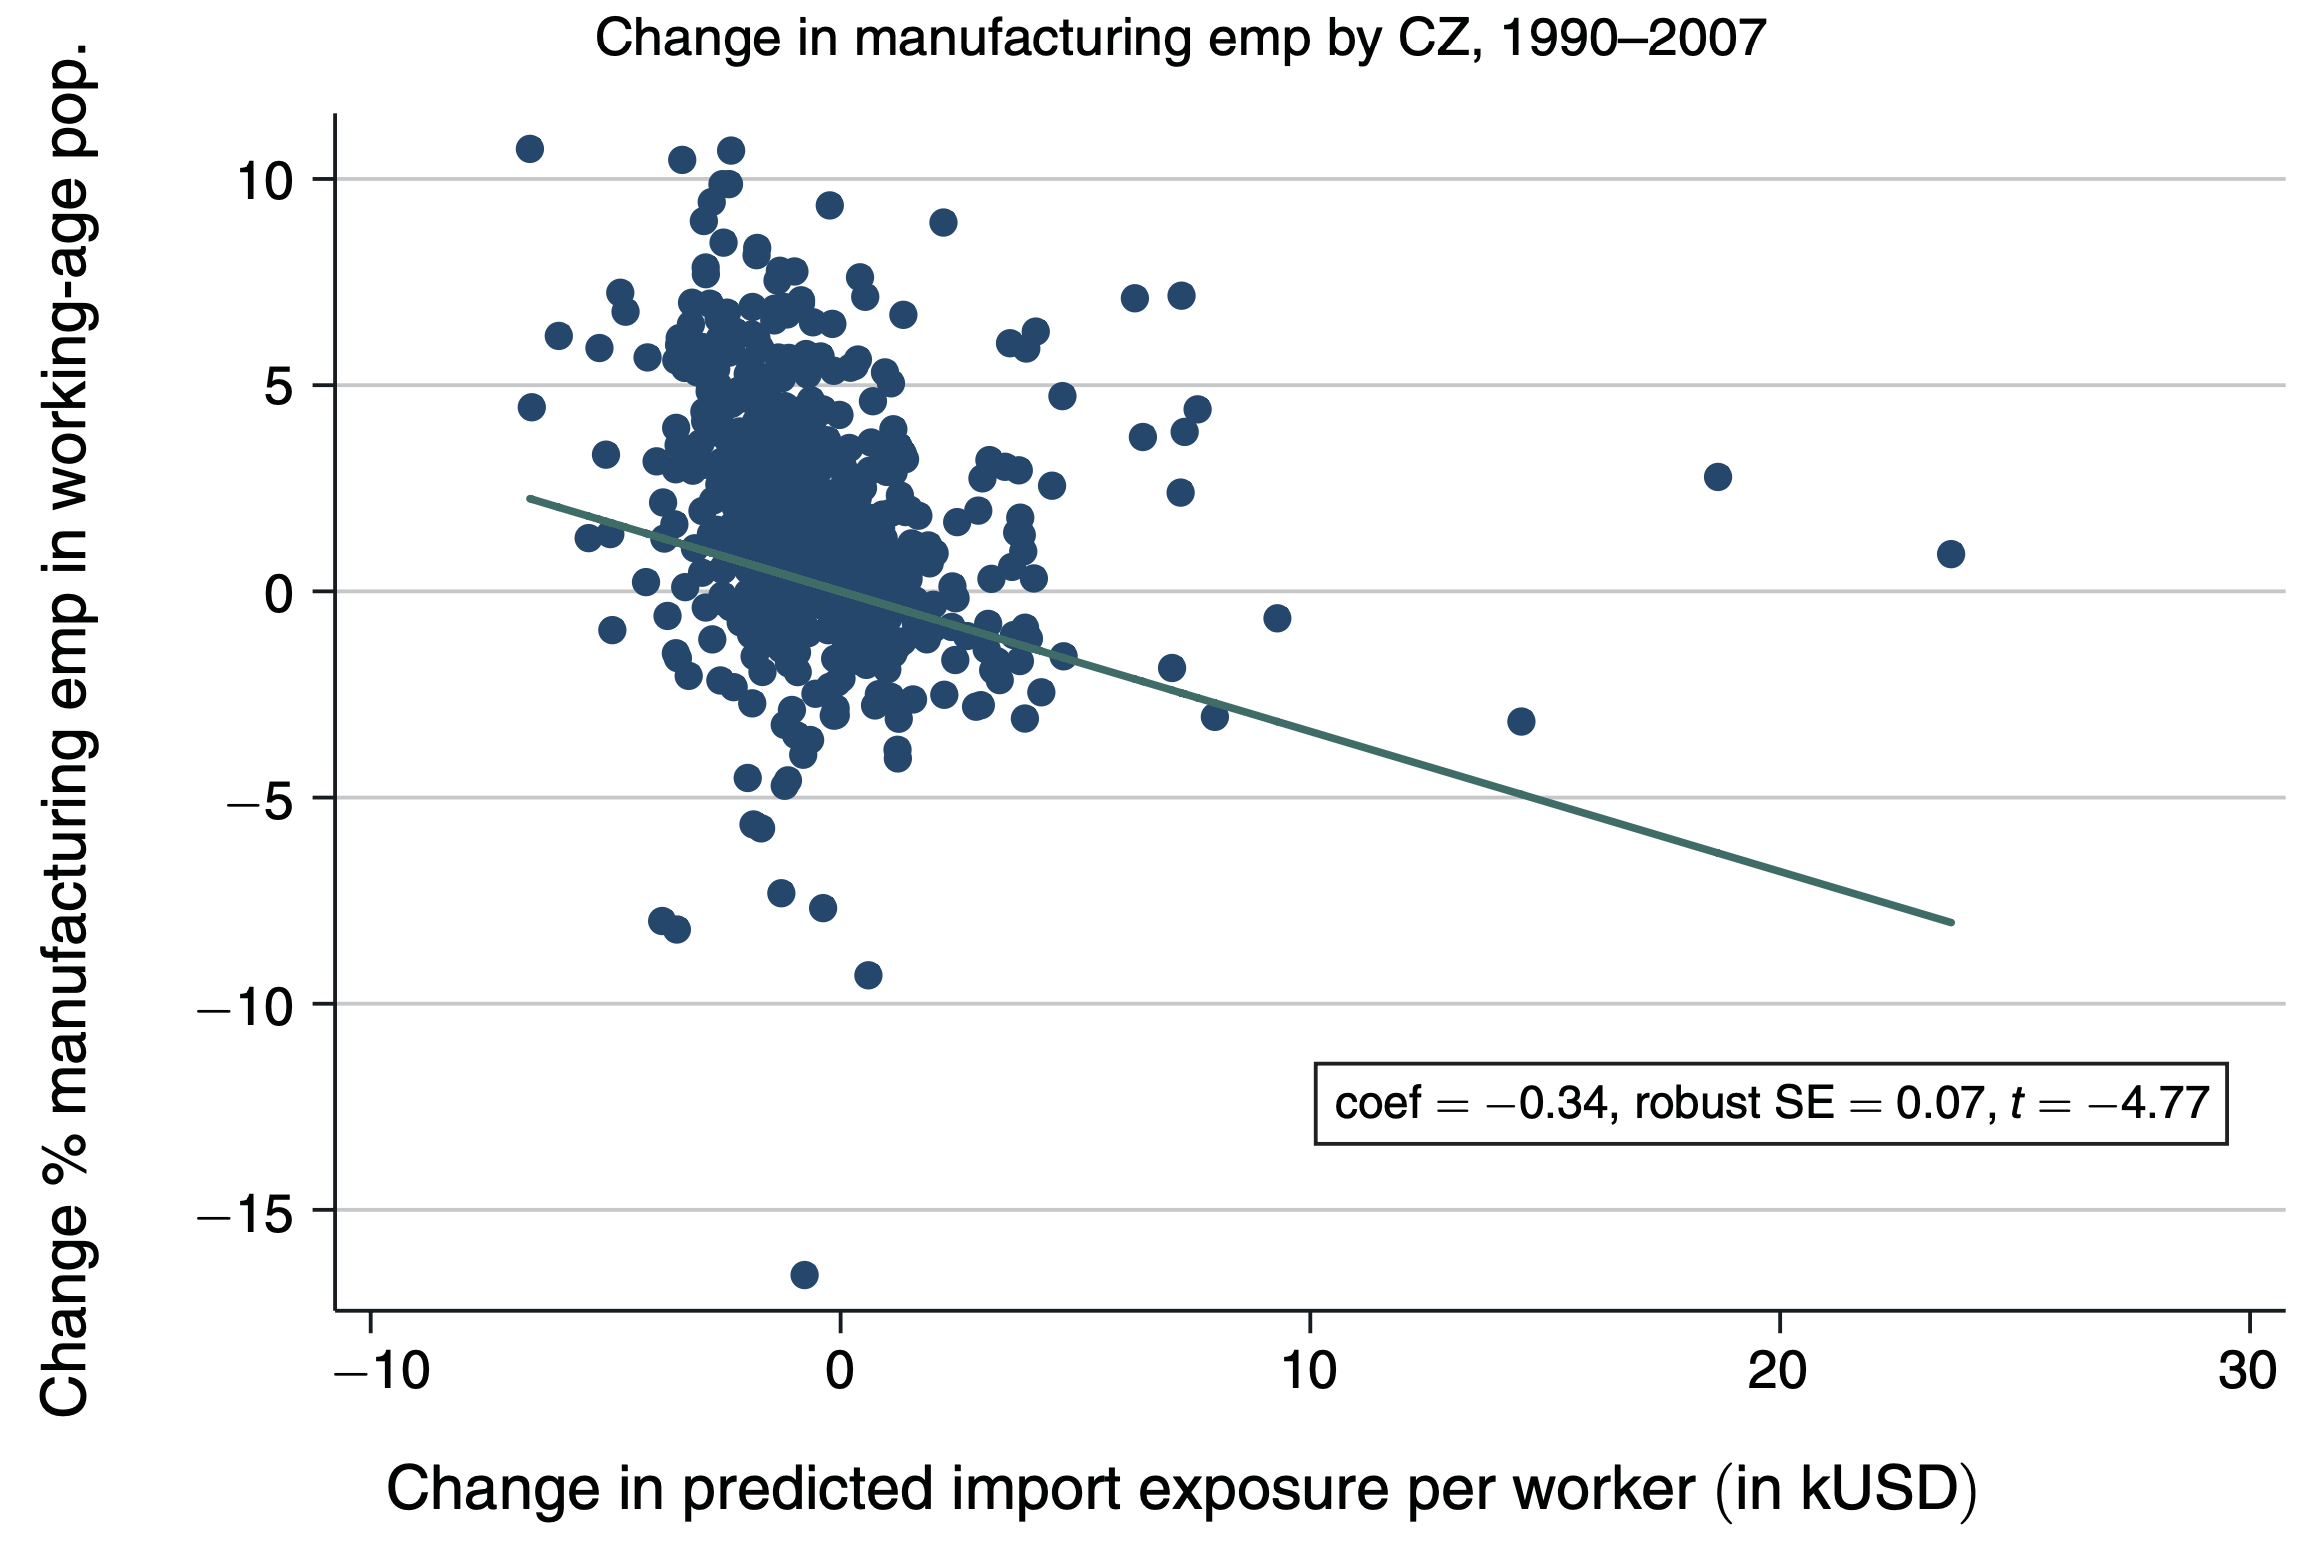
\includegraphics[width=0.8\linewidth]{Bildschirmfoto 2024-11-13 um 23.48.06.png}
        \caption{Source: \textcite{china_syndrome}}
        \label{fig:enter-label}
    \end{figure}
\end{frame}

% Slide 8 - Results: Employment Effects
\begin{frame}{Results: Employment Effects}
    \begin{itemize}
        \item \textbf{Manufacturing Decline}: Higher import exposure leads to a substantial reduction in manufacturing employment.
        \item \textbf{Example}: CZs at the 75th percentile of import exposure experienced a 4.5\% larger drop in manufacturing employment compared to those at the 25th percentile.
        \item \textbf{Broader Employment Declines}: Reduction in overall employment-to-population ratios.
    \end{itemize}
\end{frame}

% Slide 9 - Results: Wage Effects
\begin{frame}{Results: Wage Effects}
    \begin{itemize}
        \item \textbf{Wage Suppression}: Significant declines in weekly earnings in high-exposure CZs.
        \item \textbf{Heterogeneity Analysis}: Larger impact on low-skilled workers, which translates to increasing wage inequality within commuting zones.
    \end{itemize}
\end{frame}

% Slide 10 - Results: Social Transfers and Benefits
\begin{frame}{Results: Social Transfers and Benefits}
    \begin{itemize}
        \item \textbf{Increased Transfers}: Higher uptake of unemployment, disability, and welfare benefits in high-exposure regions.
        \item \textbf{Example}: CZs at the 75th percentile of import exposure experienced a 2-3.5\% rise in per capita unemployment benefits compared to those at the 25th percentile.
        \item \textbf{Implication}: Social transfer programs are implicitly used to mitigate trade-induced shocks.
    \end{itemize}
\end{frame}

% Slide 11 - Robustness Checks

% Slide 13 - Interpretation of Results
\begin{frame}{Conclusions from Results}
    \begin{itemize}
        \item \textbf{Broader Implications}: Trade with low-wage countries, like China, can exacerbate inequality within high-income countries.
        \item \textbf{Labor Market Rigidities}: Slow regional adjustments, especially for low-skilled workers, may worsen trade-related disparities through time out of the labor force.
    \end{itemize}
\end{frame}

% Slide 14 - Policy Implications
\begin{frame}{Policy Implications}
    \begin{itemize}
        \item \textbf{Trade Adjustment Assistance (TAA)}: Expand and improve TAA to address long-term impacts of trade shocks, like structural change in the manufacturing industry.
        \item \textbf{Regional Job Training Programs}: Enhance workforce development in regions heavily exposed to trade competition.
        \item \textbf{Universal Social Programs}: Broaden access to social safety nets, especially in regions facing structural trade-induced job losses.
    \end{itemize}
\end{frame}

\begin{frame}[allowframebreaks]{References}
    \printbibliography
\end{frame}


\end{document}

